\section{Module 12. Oblique imaging}

\indent The implementation of 12th module is divided in 2 parts: one part is core functions for data manipulation and the other one is visualisation. Visualisation part is also responsible for creating a new window with sliders and boxes with which it is possible to change both rotation and translation of the grid . 
\newline \indent As module input, module gets structural data as 3D array $(x, y, slice number)$. Based on this input a grid is created. For user convenience this grid is 1.2x bigger than maximum size of oblique image that can be obtained from the data. Both a shape of the data and this grid are visualized.
\newline\indent After visualisation it is possible to change rotation and translation of grid. Every change of rotation or translation automatically updates visualisation.

\begin{figure}[H]
\centering{}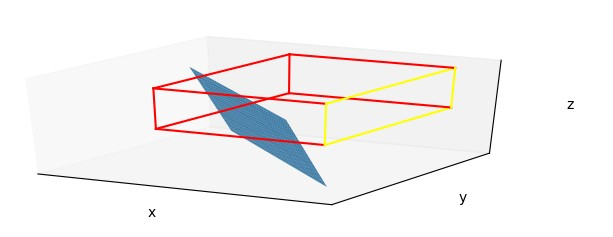
\includegraphics[scale=0.7]{figures/module_12/mod12vis}\caption{Visualization of data shape and grid \label{fig:figures/module_12/mod12vis}}
\end{figure}
\indent After clicking button 'Get oblique image' function that interpolates points needed for oblique image executes returning oblique image. 
\newline\indent Interpolation algorithm looks as follows:
\begin{itemize}
\item check if point for x,y,z from grid exists, if it exists copy values to output array
\item if not, get 8 points by rounding x,y,z grid values up and down. By that coordinates for every possible point from surroundings are gotten. Create variable for storing number of points in surroundings.
\item sum these points values
\item compute distance from interpolated point to each of those
\item if distance is longer than established (1) subtract value(s) from sum
\item divide sum of values by number of points in surroundings.
\end{itemize}
\begin{figure}[H]
\centering{}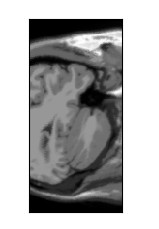
\includegraphics[scale=0.7]{figures/module_12/mod12oblim}\caption{Oblique image created based on grid shown on previous figure \label{fig:figures/module_12/mod12vis}}
\end{figure}

\indent The only library used in core part is numpy. To visualise the data matplotlib is used and PyQt is responsible for creating window.